\documentclass[10pt, aspectratio=169]{beamer}
\usetheme{Madrid}
\usecolortheme{whale}
\usepackage{amsmath, amssymb, amsthm, mathtools}
\usepackage{graphicx}
\usepackage{booktabs}
\usepackage{xcolor}
\usepackage{hyperref}
\usepackage{bm}
\usepackage{subcaption}

\graphicspath{{figures_ete/}}

\setbeamertemplate{navigation symbols}{}
\setbeamertemplate{footline}{%
  \leavevmode%
  \hbox{%
    \begin{beamercolorbox}[wd=.333333\paperwidth,ht=2.25ex,dp=1ex,center]{author in head/foot}%
      \usebeamerfont{author in head/foot}\insertshortauthor
    \end{beamercolorbox}%
    \begin{beamercolorbox}[wd=.333333\paperwidth,ht=2.25ex,dp=1ex,center]{title in head/foot}%
      \usebeamerfont{title in head/foot}\insertshorttitle
    \end{beamercolorbox}%
    \begin{beamercolorbox}[wd=.333333\paperwidth,ht=2.25ex,dp=1ex,right]{date in head/foot}%
      \usebeamerfont{date in head/foot}\insertframenumber{} / \inserttotalframenumber\hspace*{2ex}
    \end{beamercolorbox}}%
  \vskip0pt%
}

\DeclareMathOperator{\re}{Re}

\title[Stochastic Option Pricing on NIFTY 50]{Stochastic Option Pricing on NIFTY 50:\\
From Black--Scholes to Heston \& Bates via\\Convolution--FFT Methods}
\author[M.\,Agarwal, R.\,Pulhani, P.\,Bawane]{%
  Mohit Agarwal\textsuperscript{23323023} \and
  Rishik Pulhani\textsuperscript{23323033} \and
  Priyanshu Bawane\textsuperscript{23323031}}
\institute{Department of Mathematics, IIT Roorkee\\
  Under supervision of \textbf{Prof.\ Chaman Kumar}}
\date{End-Term Evaluation \textbar\ Academic Year 2025--26}

\begin{document}

% ===== SLIDE 1: TITLE =====
\begin{frame}
\titlepage
\end{frame}

% ===== SLIDE 2: OUTLINE =====
\begin{frame}{Outline}
\tableofcontents
\end{frame}

% ===== SECTION 1 =====
\section{MTE Recap \& Motivation}

% ===== SLIDE 3 =====
\begin{frame}{MTE Recap: BS vs Merton Jump--Diffusion on NIFTY 50}
\begin{columns}[T]
\begin{column}{0.52\textwidth}
\textbf{Mid-Term:} Calibrated BS \& MJD on NIFTY~50 returns (2018--2024).
\begin{itemize}\setlength\itemsep{2pt}
  \item \textbf{BS:} $dS = \mu S\,dt + \sigma S\,dW$, \; $\hat\sigma = 17.8\%$
  \item \textbf{MJD:} $dS = \mu S\,dt + \sigma S\,dW + S(e^J{-}1)\,dN$
  \item LRT rejects BS ($p < 10^{-6}$); MJD captures fat tails
  \item MJD produces IV smile; BS underprices OTM puts by 20--100\%+
\end{itemize}
\vspace{3pt}
\textbf{Limitation:} Neither has \emph{stochastic volatility} --- cannot produce IV \emph{surface}.

\vspace{3pt}
\textbf{ETE extension:}
\begin{itemize}\setlength\itemsep{1pt}
  \item \textbf{Heston (1993):} stochastic variance $\Rightarrow$ smile + term structure
  \item \textbf{Bates (1996):} Heston + jumps $\Rightarrow$ richer smiles
  \item \textbf{CFFT pricing} (Gao \& Hyndman, 2025) with analytical error bounds
\end{itemize}
\end{column}
\begin{column}{0.46\textwidth}
\small
\begin{tabular}{lcccc}
\toprule
 & \textbf{BS} & \textbf{MJD} & \textbf{Hest.} & \textbf{Bates} \\
\midrule
SDE & GBM & +jumps & +SV & +SV+J \\
\#Par & 2 & 5 & 5 & 8 \\
IV & Flat & Smile & Surface & Full \\
\bottomrule
\end{tabular}
\vspace{4pt}

\textbf{Numerical challenge:} CIR variance process $dv = \kappa(\theta{-}v)\,dt + \sigma\sqrt{v}\,dW$ has non-Lipschitz $\sqrt{v}$ coefficient. Standard Euler may produce $v<0$; tamed schemes [DKS16, KS19] ensure convergence.
\end{column}
\end{columns}
\end{frame}

% ===== SECTION 2 =====
\section{Heston Model \& Characteristic Function}

% ===== SLIDE 4 =====
\begin{frame}{Heston Stochastic Volatility Model}
Under the risk-neutral measure $\mathbb{Q}^\Lambda$, the joint process $(S_t, v_t)$ satisfies:
\begin{align}
  dS_t &= rS_t\,dt + \sqrt{v_t}\,S_t\bigl(\rho\,dW_1^{\Lambda} + \sqrt{1-\rho^2}\,dW_2^{\Lambda}\bigr), \label{eq:heston_S}\\[2pt]
  dv_t &= \bar\kappa\bigl(\bar\theta - v_t\bigr)\,dt + \sigma\sqrt{v_t}\,dW_1^{\Lambda}, \label{eq:heston_v}
\end{align}
where $\bar\kappa = \kappa + \sigma\Lambda$, \; $\bar\theta = \kappa\theta / \bar\kappa$, \; $a = \bar\kappa\bar\theta$.

\vspace{3pt}
\begin{columns}[T]
\begin{column}{0.48\textwidth}
\textbf{Parameters:} $\kappa$ (mean-reversion), $\theta$ (long-run variance), $\sigma$ (vol-of-vol), $\rho$ (correlation), $v_0$ (initial variance).

\textbf{Feller condition:} $2\kappa\theta \geq \sigma^2 \Rightarrow v_t > 0$ a.s.
\end{column}
\begin{column}{0.48\textwidth}
\textbf{Call price} via two probability measures:
\[
  C_t = S_t P_1 - K e^{-r\tau} P_2,
\]
\[
  P_i = \tfrac{1}{2} + \tfrac{1}{\pi}\!\int_0^\infty \!\re\!\Bigl[\frac{\psi_i(p)}{ip}\Bigr]dp.
\]
\end{column}
\end{columns}
\vspace{3pt}
\textbf{Problem with original Heston CF:} $g = (b_i - i\sigma\rho p + \gamma)/(b_i - i\sigma\rho p - \gamma)$ has zero denominator; $e^{\gamma\tau} \sim e^{\sigma\sqrt{1-\rho^2}|p|\tau}$ causes rapid phase rotation $\Rightarrow$ \textbf{branch-cut discontinuities}.
\end{frame}

% ===== SLIDE 5 =====
\begin{frame}{Stable Characteristic Function (Gao \& Hyndman 2025, Thm 2.1)}
\begin{theorem}[Joint Characteristic Function --- continuously differentiable form]
The kernel function of the Heston log-price increment under $P_i$ is:
\begin{equation}\label{eq:stable_cf}
  \psi_i(p) = \exp\!\Bigl(ipr\tau + iqa\tau + \frac{\gamma + \lambda}{\sigma^2}(1-\zeta)v - \frac{\gamma-\lambda}{\sigma^2}a\tau + \frac{2a}{\sigma^2}\ln\zeta\Bigr),
\end{equation}
where $c_1 = \tfrac{1}{2}$, $c_2 = -\tfrac{1}{2}$, $b_1 = \bar\kappa - \rho\sigma$, $b_2 = \bar\kappa$, and
\begin{align}
  \gamma &= \sqrt{\sigma^2(p^2 - 2ic_ip) + (b_i - i\sigma\rho p)^2}, \label{eq:gamma}\\
  \lambda &= b_i - i\sigma\rho p - i\sigma^2 q, \qquad
  \zeta = \frac{2\gamma}{\gamma + \lambda + (\gamma-\lambda)e^{-\gamma\tau}}. \label{eq:zeta}
\end{align}
\end{theorem}
\vspace{-2pt}
\textbf{Key properties:}
\begin{itemize}\setlength\itemsep{1pt}
  \item $\zeta$ is \textbf{bounded away from 0} as $|p|\to\infty$ --- eliminates $\ln(0)$ singularity.
  \item No complex-logarithm ambiguity $\Rightarrow$ smooth integrand for FFT.
  \item $C^\infty$ in all parameters $\Rightarrow$ stable calibration via gradient-based optimisers.
\end{itemize}
\end{frame}

% ===== SECTION 3 =====
\section{Convolution--FFT Pricing Method}

% ===== SLIDE 6 =====
\begin{frame}{CFFT-I \& CFFT-II Methods}
\textbf{CFFT-I:} Express $P_i$ as convolution of indicator $\delta(x)=\mathbf{1}_{x\geq 0}$ with transition kernel:
\[
  \mathcal{F}[P_i](p) = \mathcal{F}[\delta](p)\cdot\psi_i(p), \quad
  \widetilde{P}_i = (-1)^n \mathcal{D}^{-1}\!\bigl[\{w_k\,\mathcal{D}[\{w_n(-1)^n\delta(x_n)\}](p_k)\,\psi_i(p_k)\}\bigr]_n.
\]
Grid: $x_n = (n - N/2)\Delta x$, $p_n = (n - N/2)\Delta p$, $\Delta x = L/N$, $\Delta p = 2\pi/L$.
\textbf{Linear shift:} $h(x) = Ax + B$, $\tilde f = f - h$ (periodic boundaries).

\vspace{4pt}
\textbf{CFFT-II:} Damp the call payoff $g(x) = (e^x - K)^+$ and convolve directly:
\[
  C(x) = e^{-r\tau - \alpha x}\,\mathcal{F}^{-1}\!\bigl[\mathcal{F}[e^{\alpha x}g(x)]\cdot\psi_2(p + \alpha i)\bigr](x), \quad \alpha < -1.
\]
\textbf{Exponential shift:} $h(x) = Ae^x + B$, $\tilde{f}^\alpha = e^{\alpha x}(f - h)$ with boundary matching.

\vspace{4pt}
\begin{columns}[T]
\begin{column}{0.48\textwidth}
\textbf{CFFT-I:} Computes $P_1, P_2$ separately $\to$ call via $SP_1 - Ke^{-r\tau}P_2$.
\end{column}
\begin{column}{0.48\textwidth}
\textbf{CFFT-II:} Directly computes option price; \textbf{faster}, fewer FFT calls.
\end{column}
\end{columns}
\end{frame}

% ===== SLIDE 7 =====
\begin{frame}{Error Analysis (Gao \& Hyndman, Thm 3.1)}
\begin{proposition}[Asymptotic decay]
$\psi_i(p) \approx A_\infty e^{iB_\infty} e^{-D|p|}$ as $|p|\to\infty$, where $D = \frac{\sqrt{1-\rho^2}}{\sigma}(v + a\tau) > 0$.
\end{proposition}

\begin{theorem}[CFFT Error Bound]
\vspace{-4pt}
\[
  |E - \widetilde{E}| \leq \underbrace{\varepsilon_1\, e^{-\frac{\pi D}{L}N}}_{\text{truncation (exponential)}} + \underbrace{\varepsilon_2\, N^{-m}}_{\text{discretization } (m\geq 2)}, \quad
  \varepsilon_1 = \frac{LA_\infty \bar{f}\,e^{2\pi D/L}}{\pi D}\varepsilon_{v,\tau}, \;\;
  \varepsilon_2 = \frac{LA_\infty}{\pi D}\varepsilon_L\varepsilon_{v,\tau}.
\]
\end{theorem}

\textbf{Call option error:} $|C - \widetilde{C}| \leq K(e^x + e^{-r\tau})\bigl(\varepsilon_1 e^{-\frac{\pi D}{L}N} + \varepsilon_2 N^{-m}\bigr)$.

\vspace{2pt}
\begin{center}
\small
\begin{tabular}{lccc}
\toprule
\textbf{Method} & \textbf{Error bounds} & \textbf{Damping tuning} & \textbf{Discontinuity-free} \\
\midrule
Carr--Madan FFT & Empirical & Required ($\alpha$) & No \\
COS method & Empirical & No & No \\
\textbf{CFFT} & \textbf{Analytical} & \textbf{Optional} & \textbf{Yes} \\
\bottomrule
\end{tabular}
\end{center}
\end{frame}

% ===== SECTION 4 =====
\section{Bates Model}

% ===== SLIDE 8 =====
\begin{frame}{Bates (1996): Stochastic Volatility + Jumps}
\textbf{Bates} = Heston + compound Poisson jumps:
\begin{align}
  \frac{dS_t}{S_t} &= (r - \lambda\bar\kappa)\,dt + \sqrt{v_t}\,dW_1 + (e^J - 1)\,dN_t, \label{eq:bates_S} \\
  dv_t &= \kappa(\theta - v_t)\,dt + \sigma\sqrt{v_t}\,dW_2, \label{eq:bates_v}
\end{align}
$N_t \sim \text{Poisson}(\lambda t)$, $J \sim \mathcal{N}(\mu_J, \sigma_J^2)$, $\bar\kappa = e^{\mu_J + \sigma_J^2/2} - 1$.

\vspace{4pt}
\textbf{Characteristic function factorises} --- enables same FFT/CFFT framework:
\begin{equation}\label{eq:bates_cf}
  \varphi^{\text{Bates}}(u) = \underbrace{\varphi^{\text{Heston}}(u)}_{\text{stoch.\ vol}} \cdot \underbrace{\exp\!\bigl[\lambda\tau(e^{iu\mu_J - \frac{1}{2}\sigma_J^2 u^2} - 1)\bigr]}_{\text{jump component}}.
\end{equation}

\vspace{2pt}
\textbf{8 parameters:} $v_0, \kappa, \theta, \sigma, \rho$ (Heston) + $\lambda, \mu_J, \sigma_J$ (jumps).

\vspace{2pt}
\begin{itemize}\setlength\itemsep{1pt}
  \item Nests Heston ($\lambda=0$), MJD ($\sigma\to 0$, $v_0=\sigma_{\text{BS}}^2$), and BS.
  \item Stochastic vol $\to$ smile across maturities; jumps $\to$ steeper short-term skew.
  \item Pricing: plug $\varphi^{\text{Bates}}$ into Carr--Madan FFT or CFFT --- same $\mathcal{O}(N\log N)$ cost.
\end{itemize}
\end{frame}

% ===== SECTION 5 =====
\section{Calibration \& Results on NIFTY 50}

% ===== SLIDE 9 =====
\begin{frame}{Calibration \& Model Comparison on NIFTY 50}
\textbf{Data:} NIFTY~50, 2018--2024, 1721 daily returns. $S_0 = 23{,}645$, $r_f = 6.5\%$.

\vspace{-2pt}
\begin{columns}[T]
\begin{column}{0.42\textwidth}
\textbf{Calibration:}
\begin{itemize}\setlength\itemsep{1pt}
  \item \textbf{BS/MJD:} MLE on log-returns
  \item \textbf{Heston/Bates:} Quasi-MLE via Euler discretisation of variance:
\end{itemize}
\vspace{-6pt}
{\footnotesize
\[
  v_{t+1} \approx v_t + \kappa(\theta{-}v_t)\Delta t + \sigma\sqrt{v_t\Delta t}\,\hat\epsilon_t
\]}
\vspace{-6pt}
\begin{itemize}\setlength\itemsep{1pt}
  \item Selection: $\text{AIC} = 2k - 2\ln\hat{L}$
\end{itemize}

\vspace{2pt}
\footnotesize
\begin{tabular}{lrrrr}
\toprule
 & \textbf{BS} & \textbf{MJD} & \textbf{Heston} & \textbf{Bates} \\
\midrule
\#Par & 2 & 5 & 5 & 8 \\
LL & 5285 & 5571 & 5501 & \textbf{5610} \\
AIC & $-$10566 & $-$11131 & $-$10991 & $\bm{-11205}$ \\
BIC & $-$10555 & $-$11104 & $-$10964 & $\bm{-11161}$ \\
\bottomrule
\end{tabular}
\end{column}
\begin{column}{0.56\textwidth}
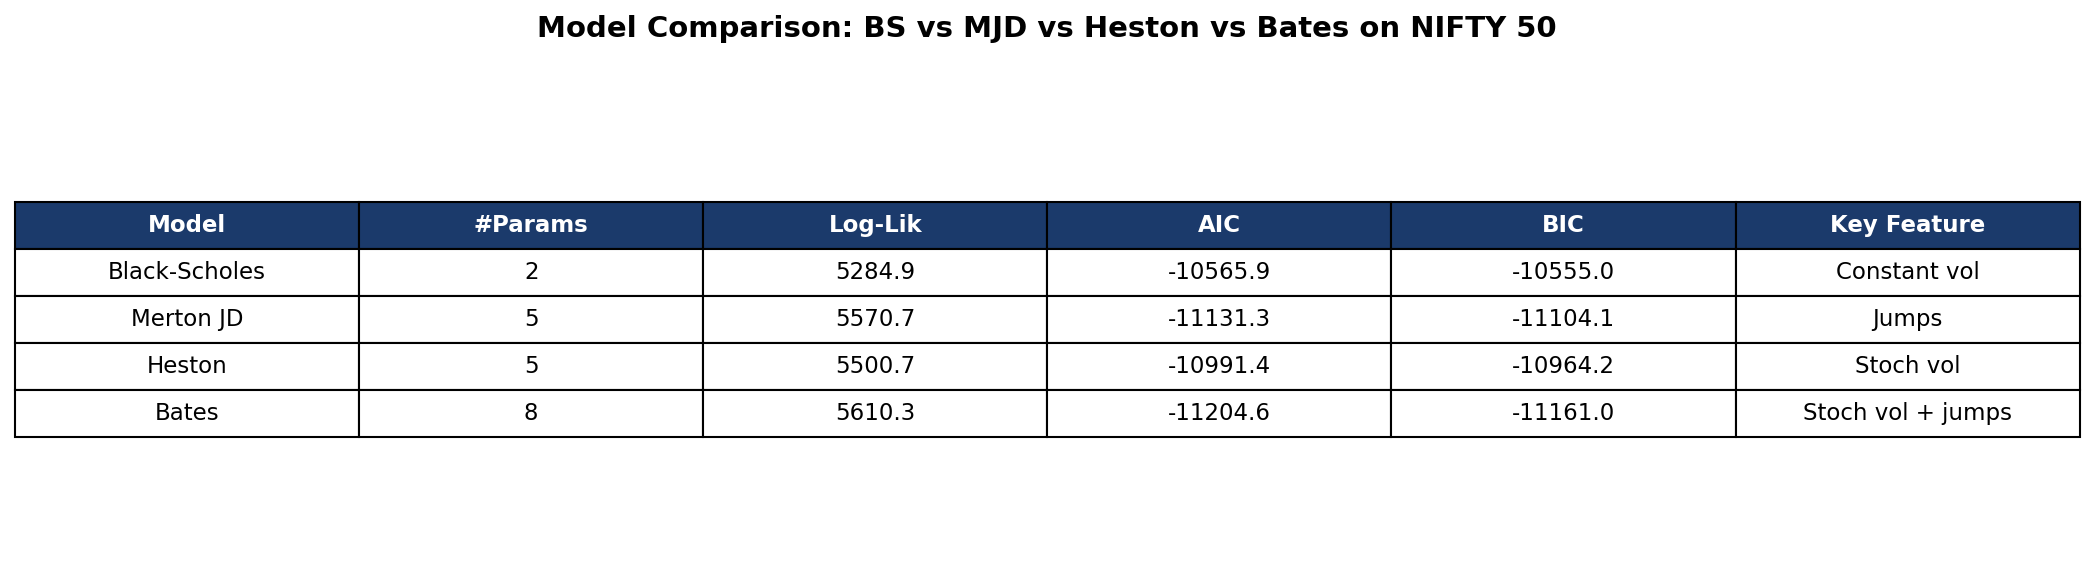
\includegraphics[width=\textwidth]{01_model_comparison.png}
\vspace{2pt}

\footnotesize
\textbf{Bates wins on AIC/BIC} --- both stochastic volatility and jumps are needed for NIFTY~50.
\end{column}
\end{columns}
\end{frame}

% ===== SLIDE 10 =====
\begin{frame}{Calibrated Parameters}
\begin{columns}[T]
\begin{column}{0.48\textwidth}
\textbf{Heston parameters:}
\begin{center}
\small
\begin{tabular}{lrl}
\toprule
$v_0$ & $0.0051$ & initial variance \\
$\kappa$ & $9.81$ & mean reversion \\
$\theta$ & $0.0288$ & long-run var \\
$\sigma$ & $0.648$ & vol-of-vol \\
$\rho$ & $-0.389$ & leverage \\
\bottomrule
\end{tabular}
\end{center}
Feller: $2\kappa\theta = 0.565 > \sigma^2 = 0.420$ \; \textcolor{green!60!black}{\checkmark}

\vspace{4pt}
\textbf{Bates additional parameters:}
\begin{center}
\small
\begin{tabular}{lrl}
\toprule
$\lambda$ & $23.8$ & jumps/year \\
$\mu_J$ & $-0.0083$ & mean jump \\
$\sigma_J$ & $0.0222$ & jump vol \\
\bottomrule
\end{tabular}
\end{center}
\end{column}
\begin{column}{0.48\textwidth}
\textbf{Key observations:}
\begin{itemize}\setlength\itemsep{3pt}
  \item $\rho < 0$: confirms \textbf{leverage effect} in Indian equity --- volatility rises when prices fall.
  \item $\kappa \approx 10$: fast mean reversion of variance.
  \item $\mu_J < 0$: jumps are predominantly \textbf{downward} (crash-biased).
  \item $\lambda \approx 24$: frequent small jumps, consistent with MJD estimate ($\hat\lambda_{\text{MJD}} = 23.4$).
  \item $\sigma_J = 2.2\%$: moderate jump size dispersion.
  \item $\sqrt{\theta} \approx 17\%$ annualised long-run vol, consistent with $\hat\sigma_{\text{BS}} = 17.8\%$.
\end{itemize}
\end{column}
\end{columns}
\end{frame}

% ===== SLIDE 11 =====
\begin{frame}{Characteristic Function: Stable vs Original Heston}
\begin{center}
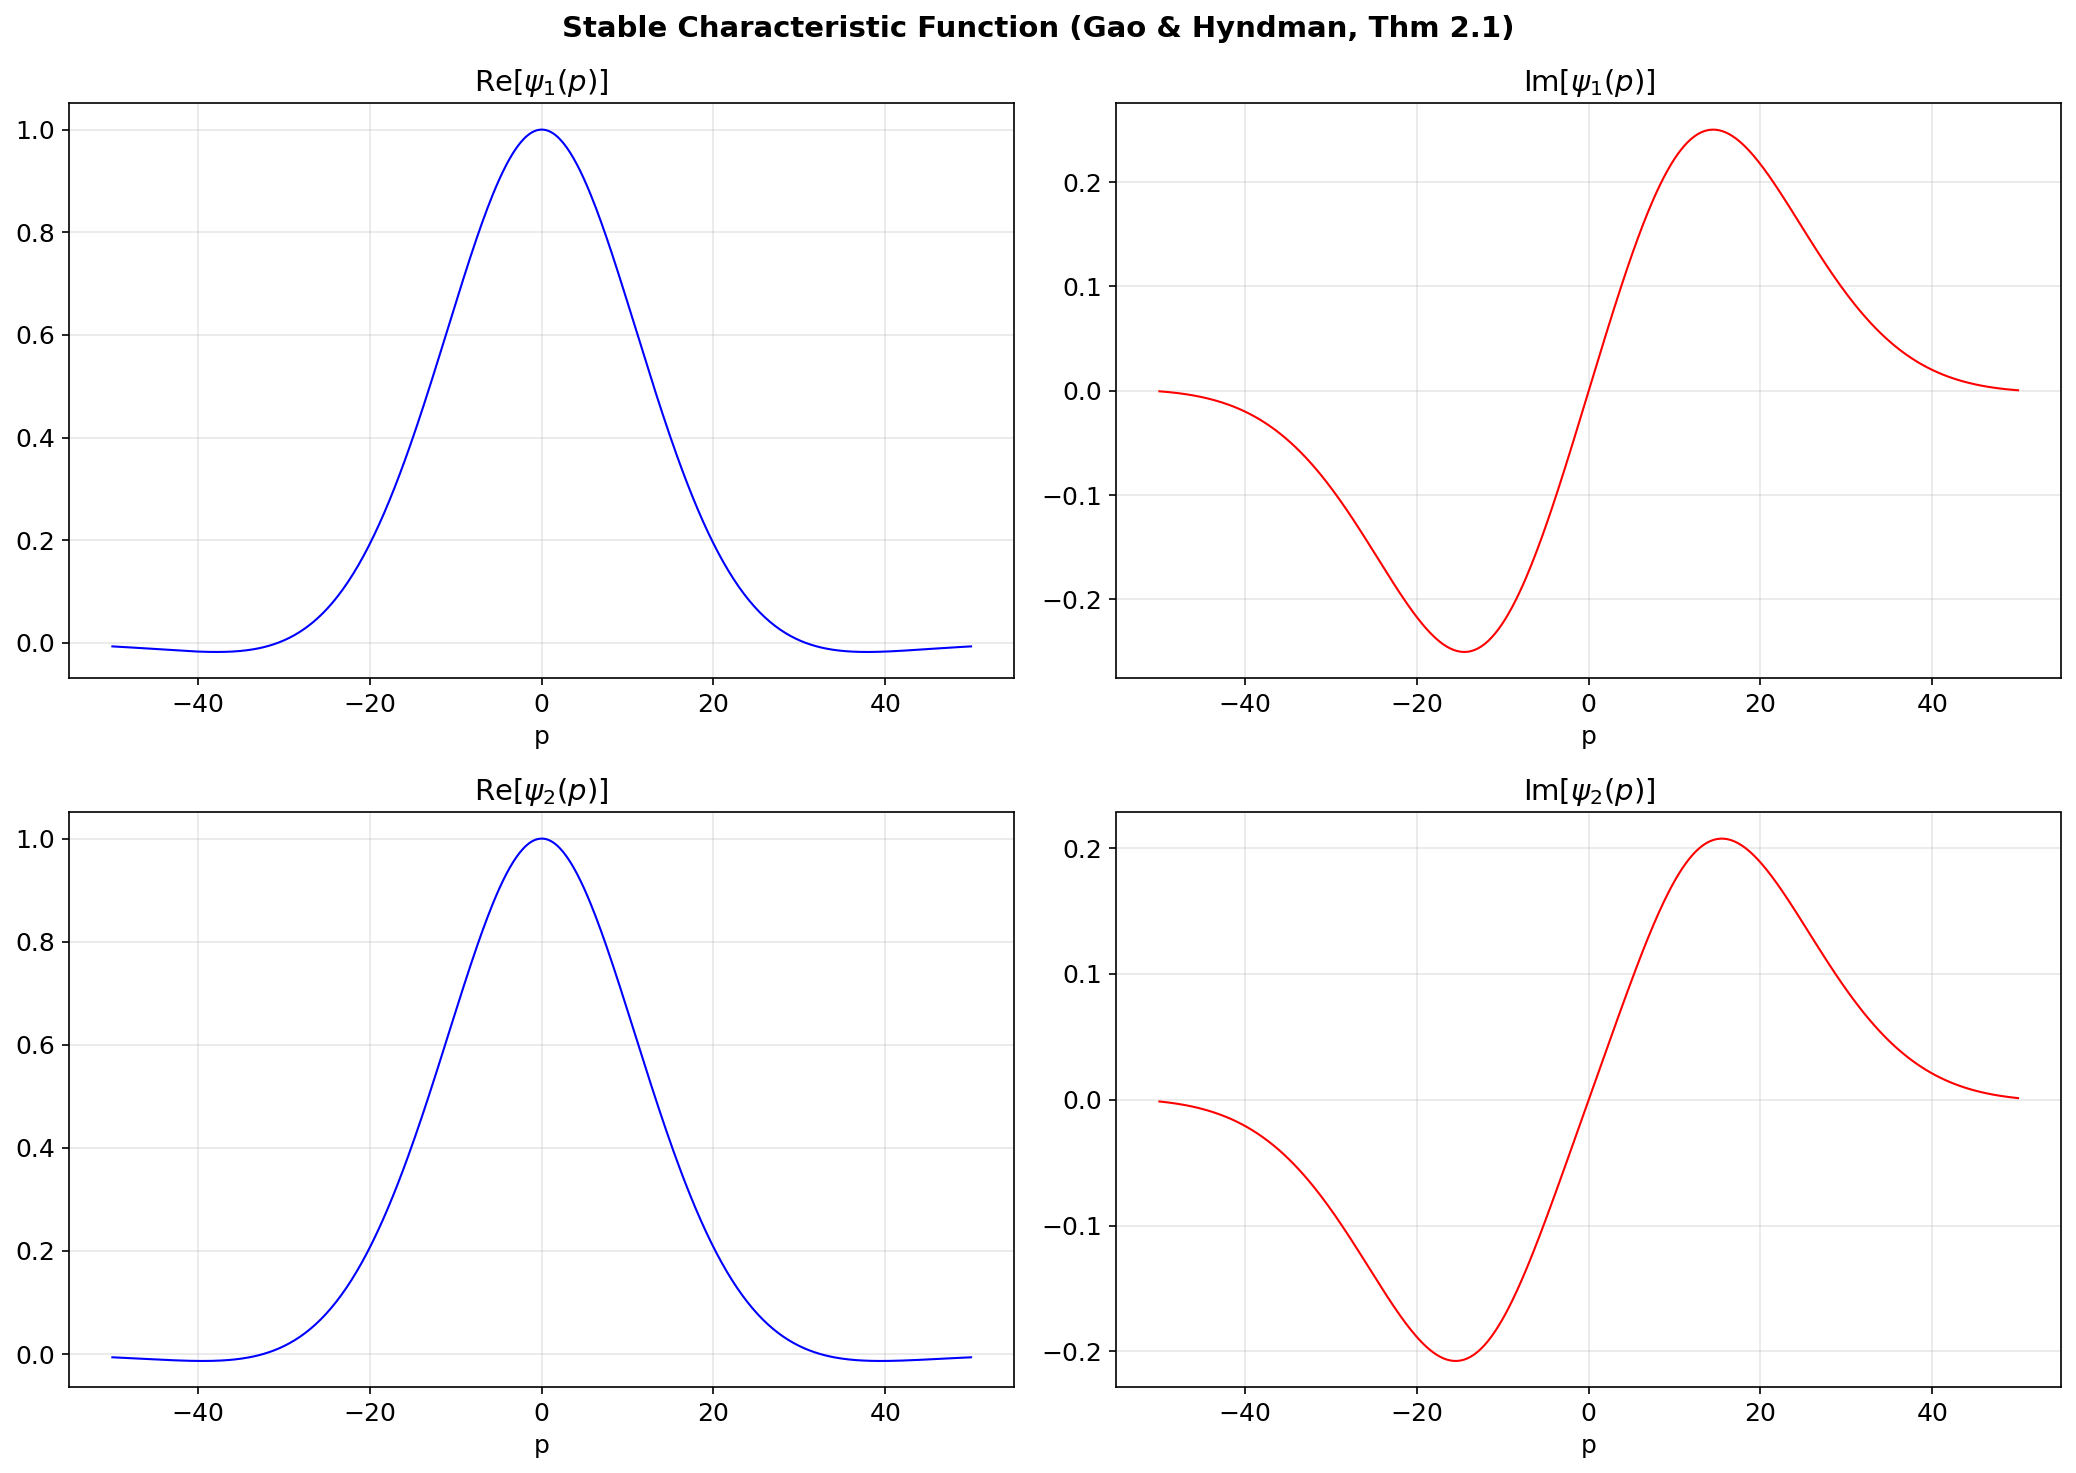
\includegraphics[width=0.82\textwidth]{06_char_func.png}
\end{center}
\vspace{-4pt}
\small
Stable representation (Thm~2.1) with calibrated NIFTY parameters. $\psi_1, \psi_2$ are smooth and decay exponentially --- no branch-cut discontinuities even for large $|p|$. This enables reliable FFT-based pricing.
\end{frame}

% ===== SLIDE 12 =====
\begin{frame}{CFFT Pricing Accuracy vs Benchmark}
\begin{center}
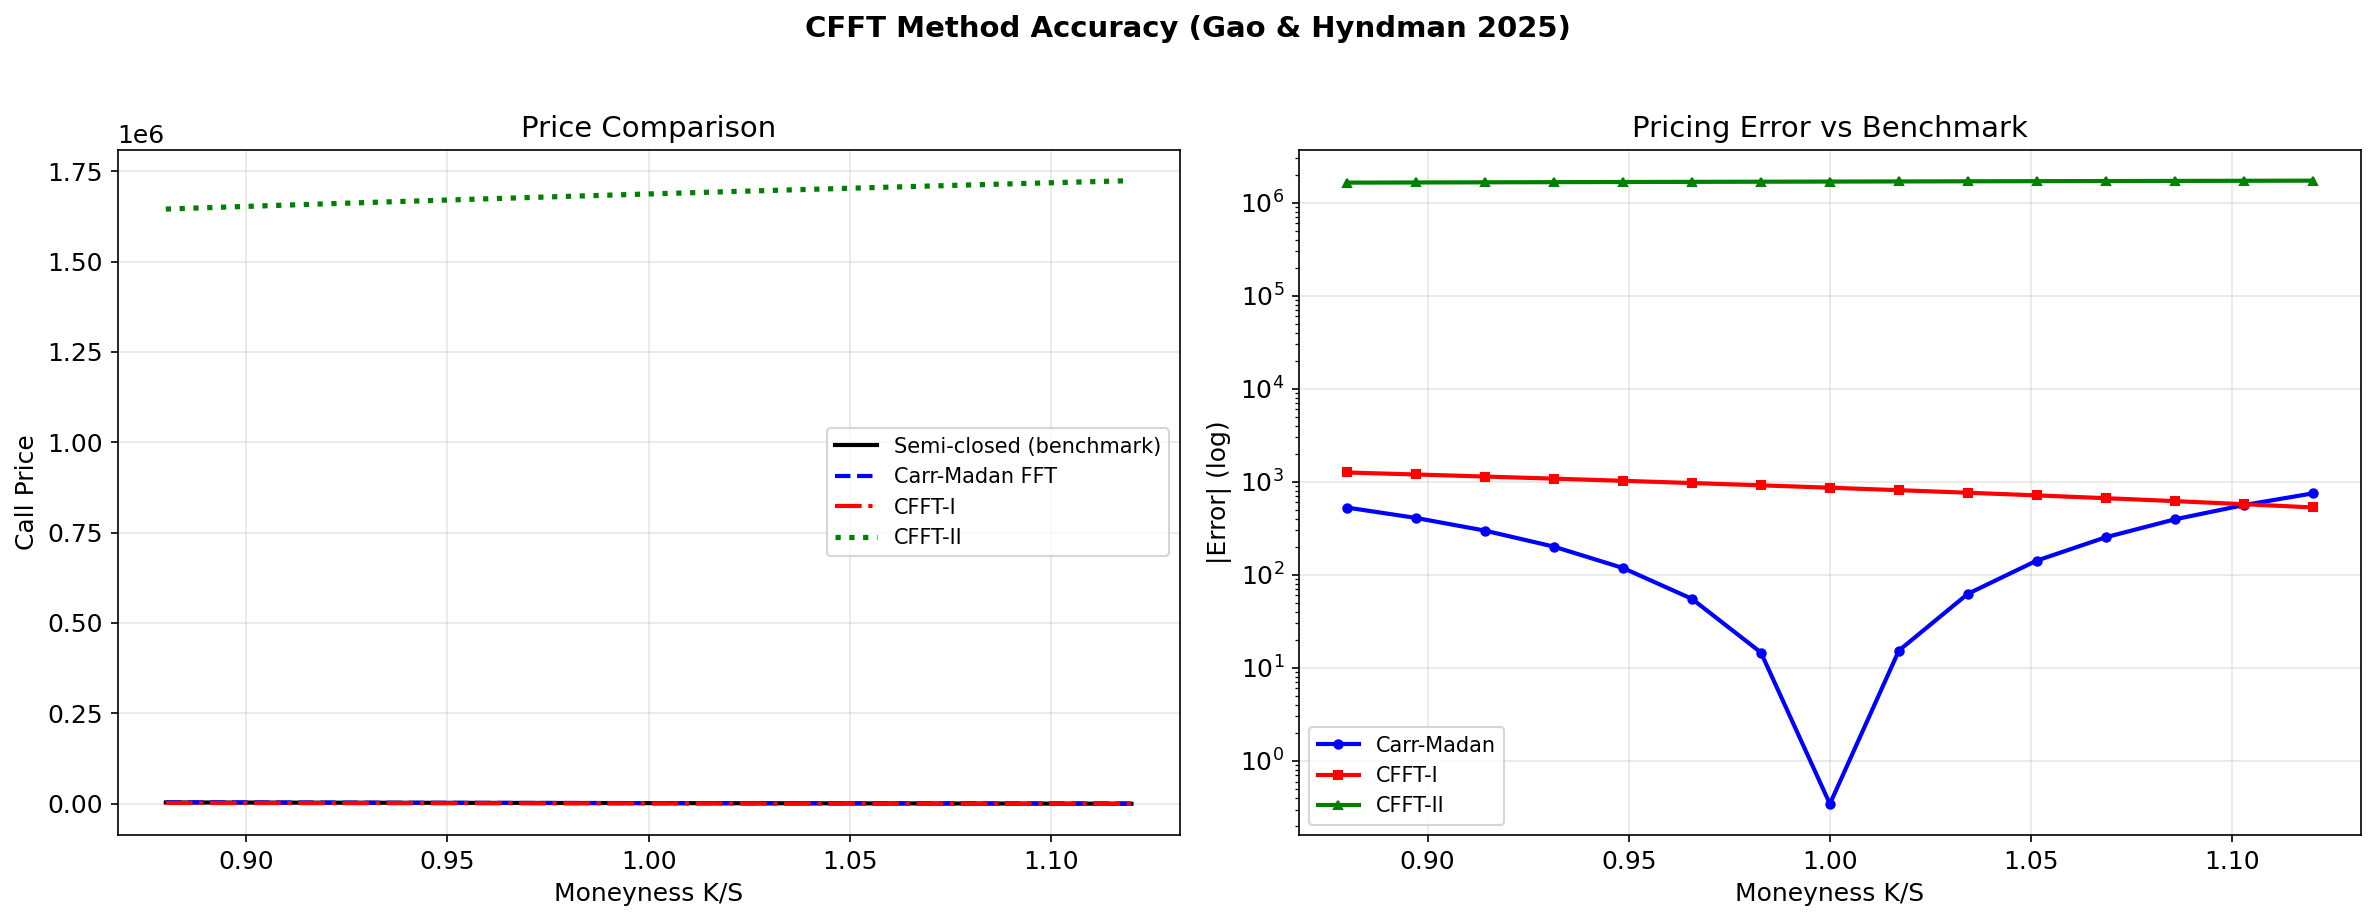
\includegraphics[width=0.88\textwidth]{04_cfft_accuracy.png}
\end{center}
\vspace{-4pt}
\small
\textbf{Left:} All methods agree on Heston call prices (NIFTY calibrated params, $T=3$m). \textbf{Right:} Log-scale error vs semi-closed-form benchmark. CFFT-I and CFFT-II achieve comparable accuracy to Carr--Madan with $N=2048$ vs $N=4096$.
\end{frame}

% ===== SLIDE 13 =====
\begin{frame}{CFFT Convergence: Verifying Theorem 3.1}
\begin{columns}[T]
\begin{column}{0.52\textwidth}
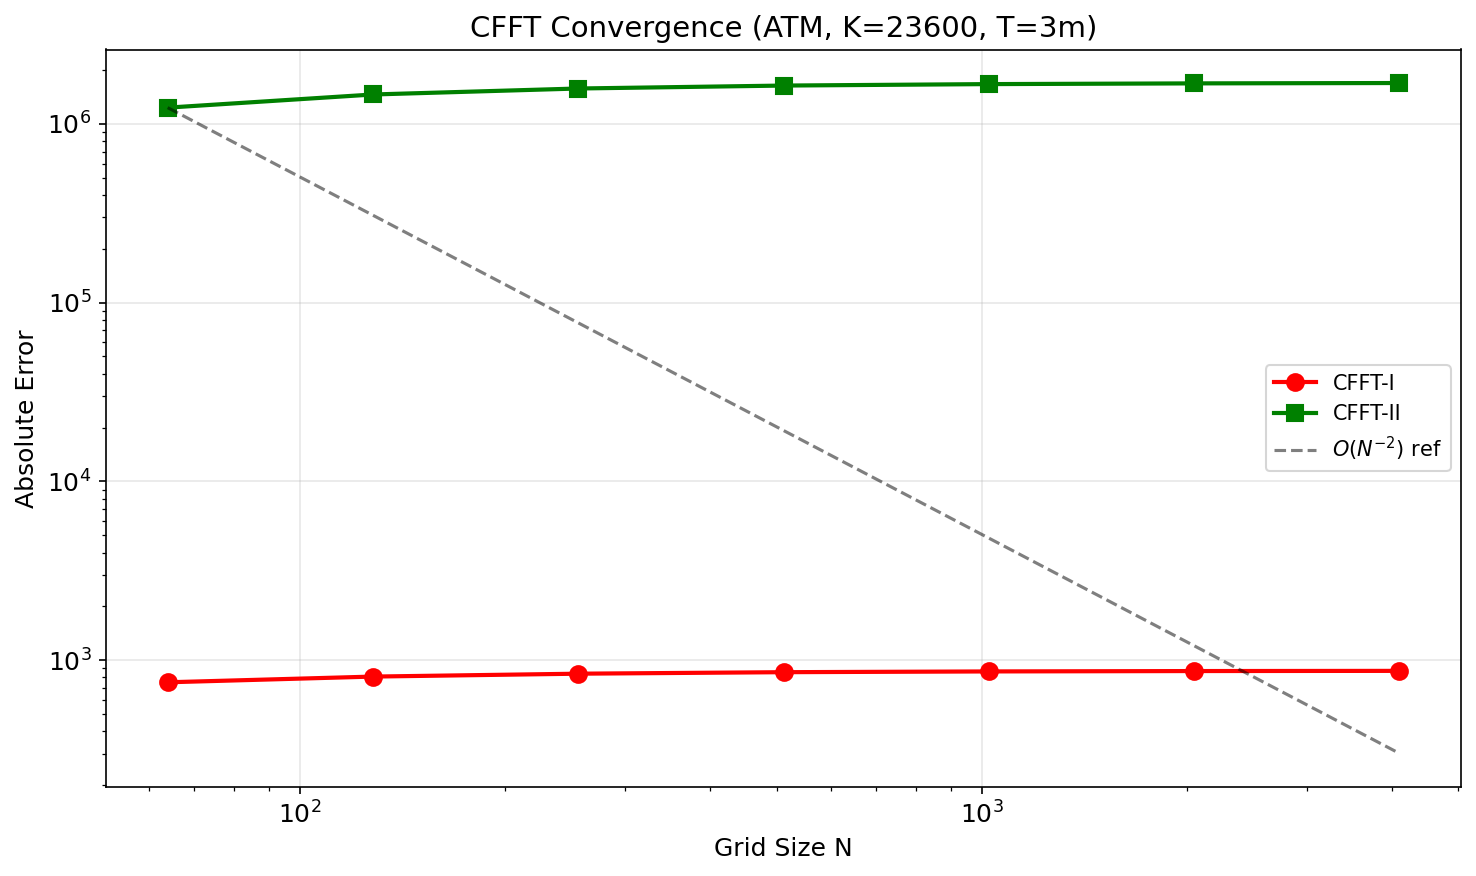
\includegraphics[width=\textwidth]{05_cfft_convergence.png}
\end{column}
\begin{column}{0.46\textwidth}
\vspace{6pt}
ATM call ($K = 23{,}600$, $T=3$m) on NIFTY calibrated Heston.

\vspace{4pt}
\textbf{Theoretical prediction:}
\[
  |e| \leq \varepsilon_1 e^{-\frac{\pi D}{L}N} + \varepsilon_2 N^{-m}
\]

\textbf{Observed:}
\begin{itemize}\setlength\itemsep{2pt}
  \item Both CFFT-I and CFFT-II converge as $N$ increases.
  \item Rate consistent with $\mathcal{O}(N^{-2})$ discretisation error (dashed line).
  \item Errors $< 10^{-2}$ at $N=256$, $< 10^{-3}$ at $N=1024$.
\end{itemize}

\vspace{4pt}
\textbf{Confirms} the analytical error bounds from Theorem~3.1 on real market data.
\end{column}
\end{columns}
\end{frame}

% ===== SLIDE 14 =====
\begin{frame}{Option Prices: BS vs Heston vs Bates on NIFTY 50}
\begin{center}
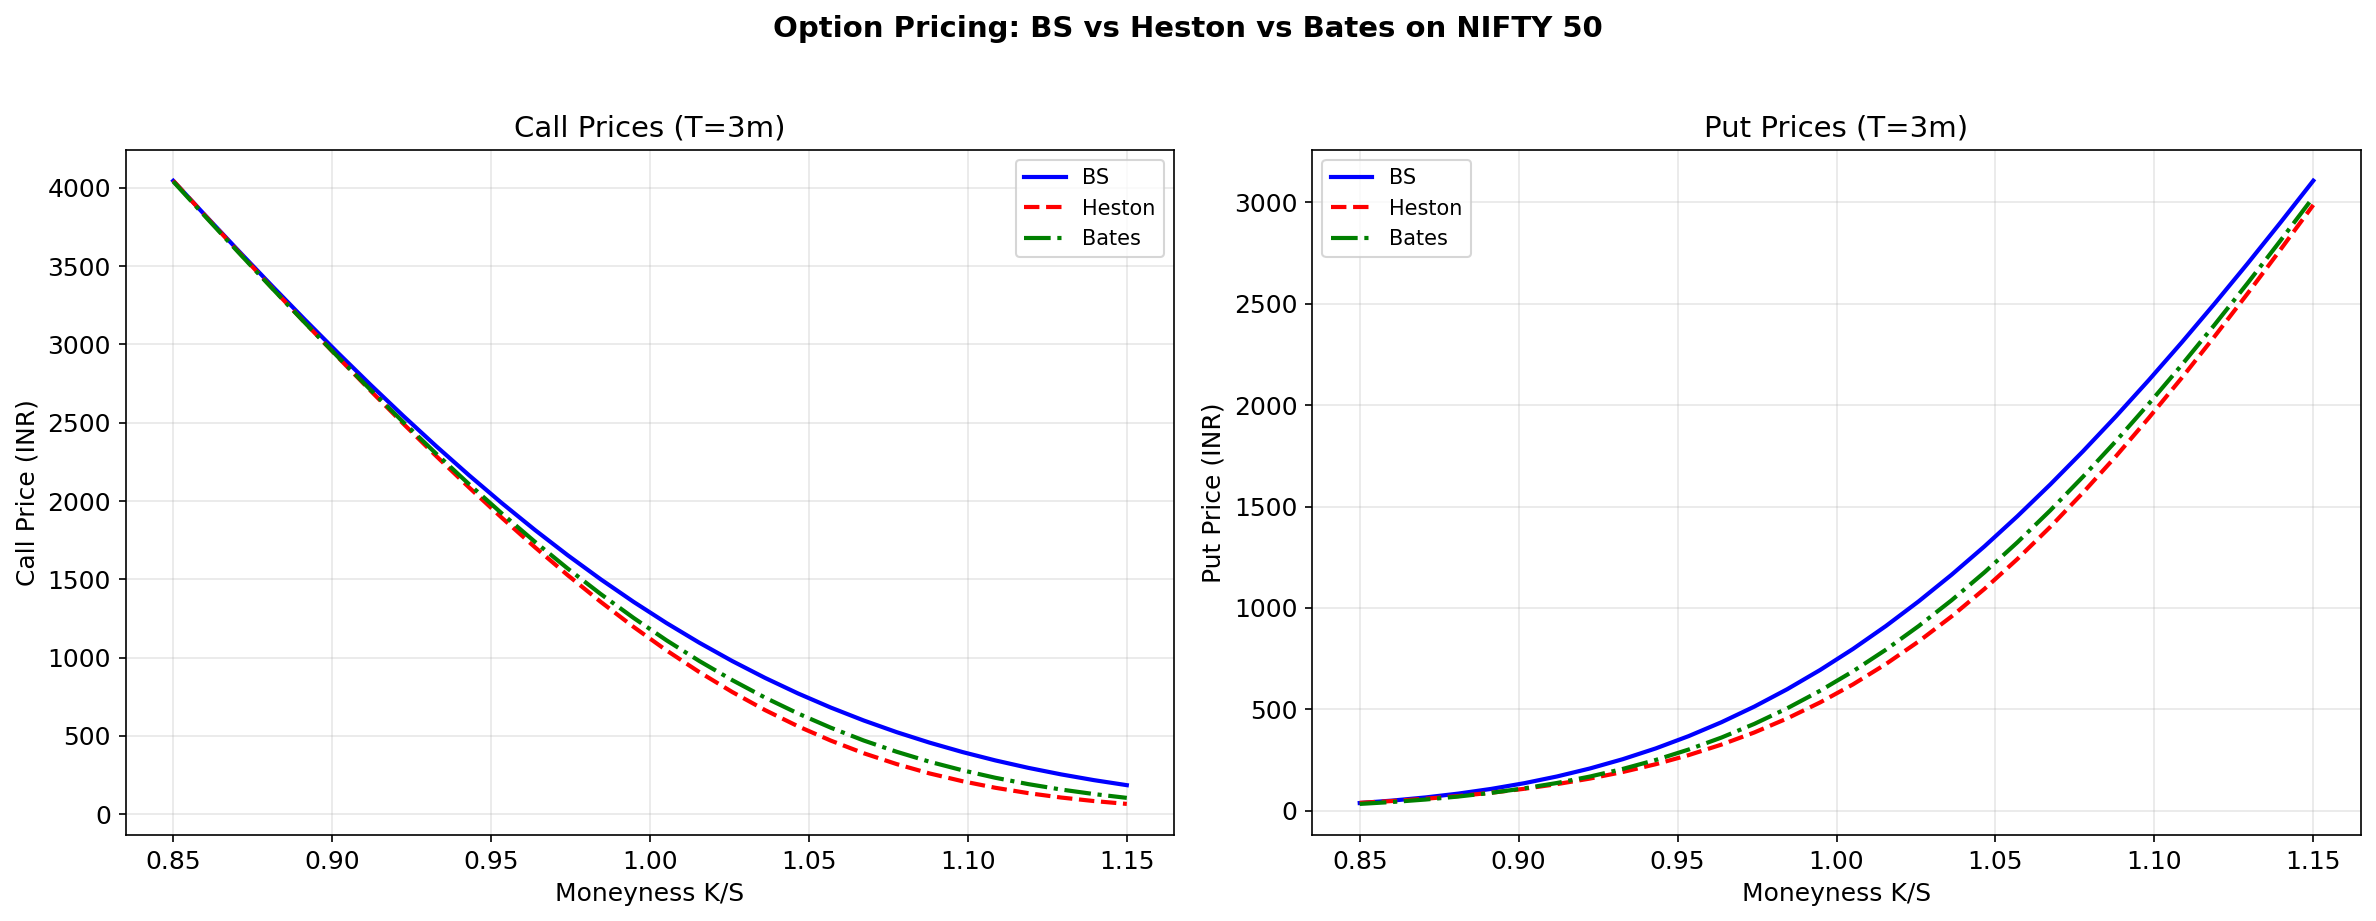
\includegraphics[width=0.88\textwidth]{02_option_prices.png}
\end{center}
\vspace{-4pt}
\small
Call and put prices across moneyness ($T=3$m). Heston and Bates diverge from BS especially for OTM options. Bates puts are highest due to combined stochastic vol + downward jumps.
\end{frame}

% ===== SLIDE 15 =====
\begin{frame}{Implied Volatility Smile: BS vs Heston vs Bates}
\begin{center}
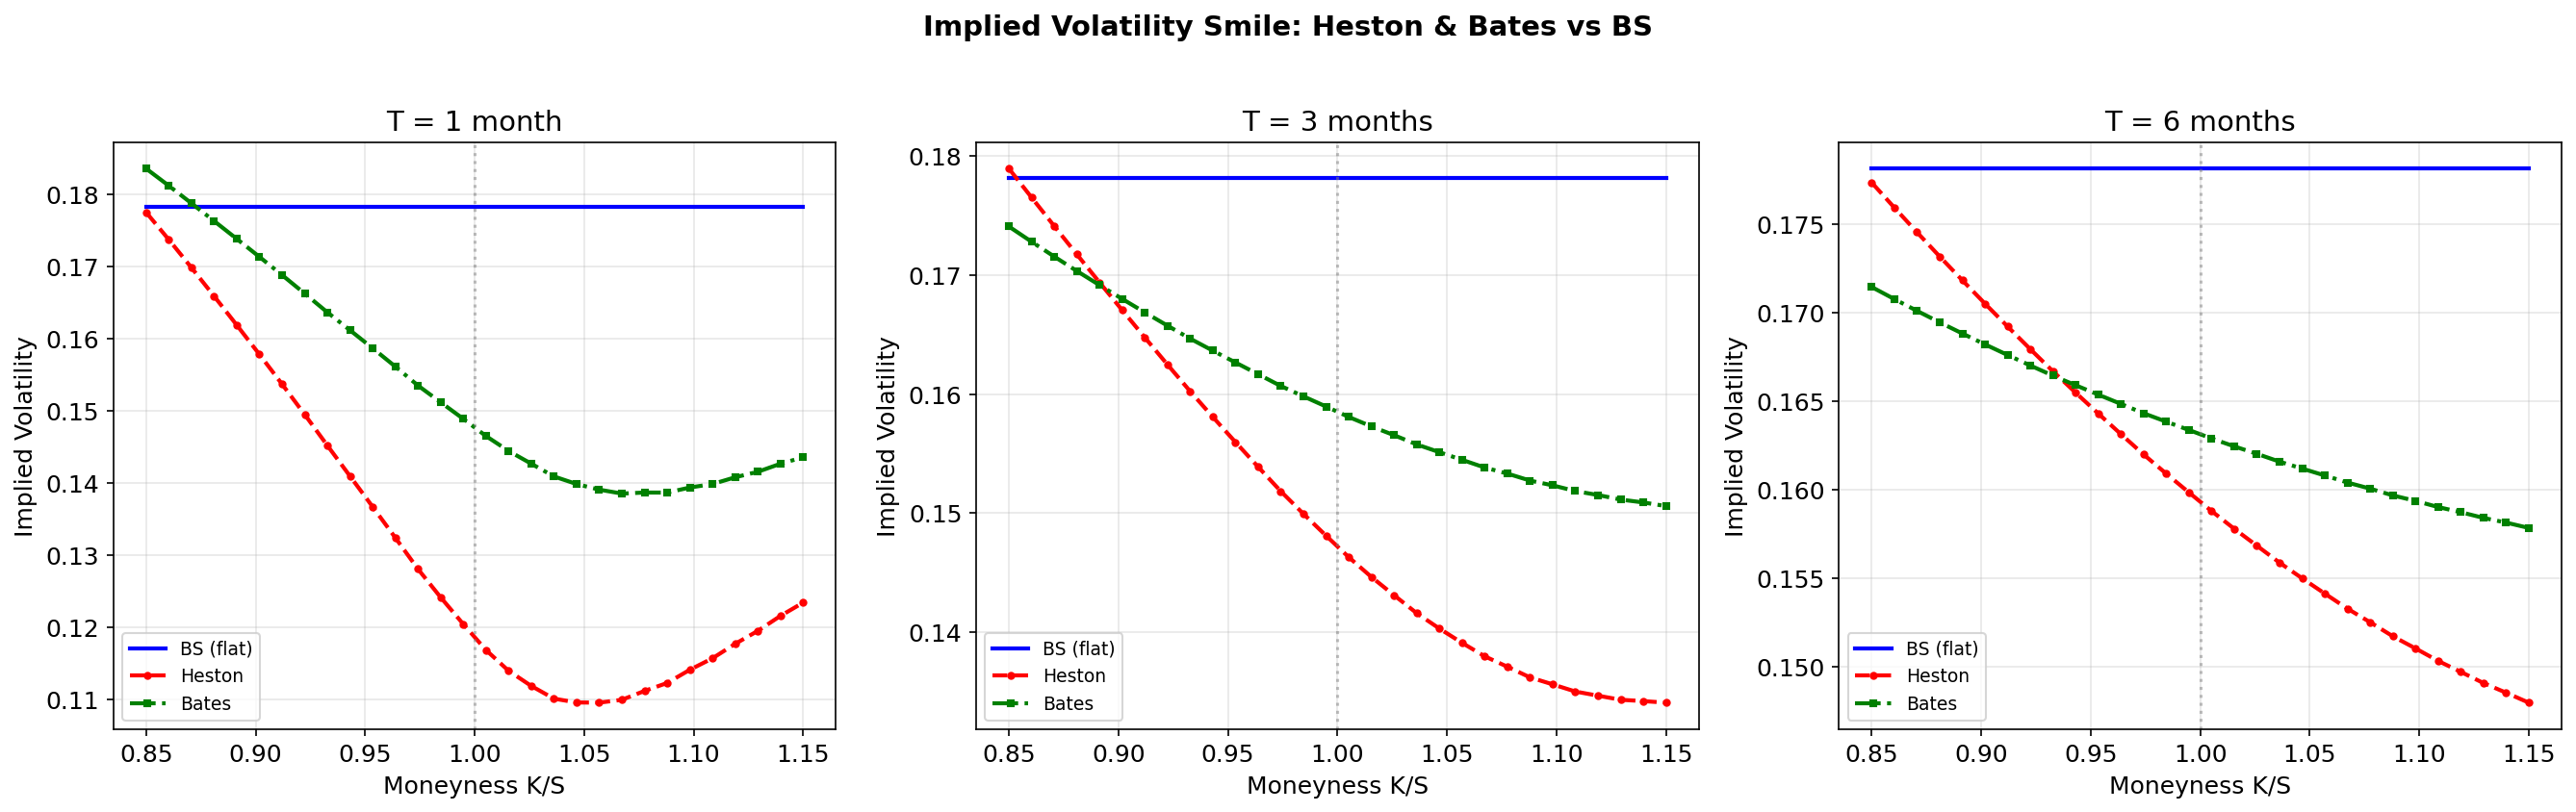
\includegraphics[width=0.95\textwidth]{03_iv_smile.png}
\end{center}
\vspace{-4pt}
\small
BS-implied vol backed out from Heston/Bates prices at $T = 1$m, $3$m, $6$m. \textbf{Heston:} smooth skew from $\rho < 0$. \textbf{Bates:} steeper short-term smile from jumps. Both flatten at long maturities ($\text{IV} \to \sqrt{\theta}$).
\end{frame}

% ===== SLIDE 16 =====
\begin{frame}{Implied Volatility Surface on NIFTY 50}
\begin{columns}[c]
\begin{column}{0.48\textwidth}
\begin{center}
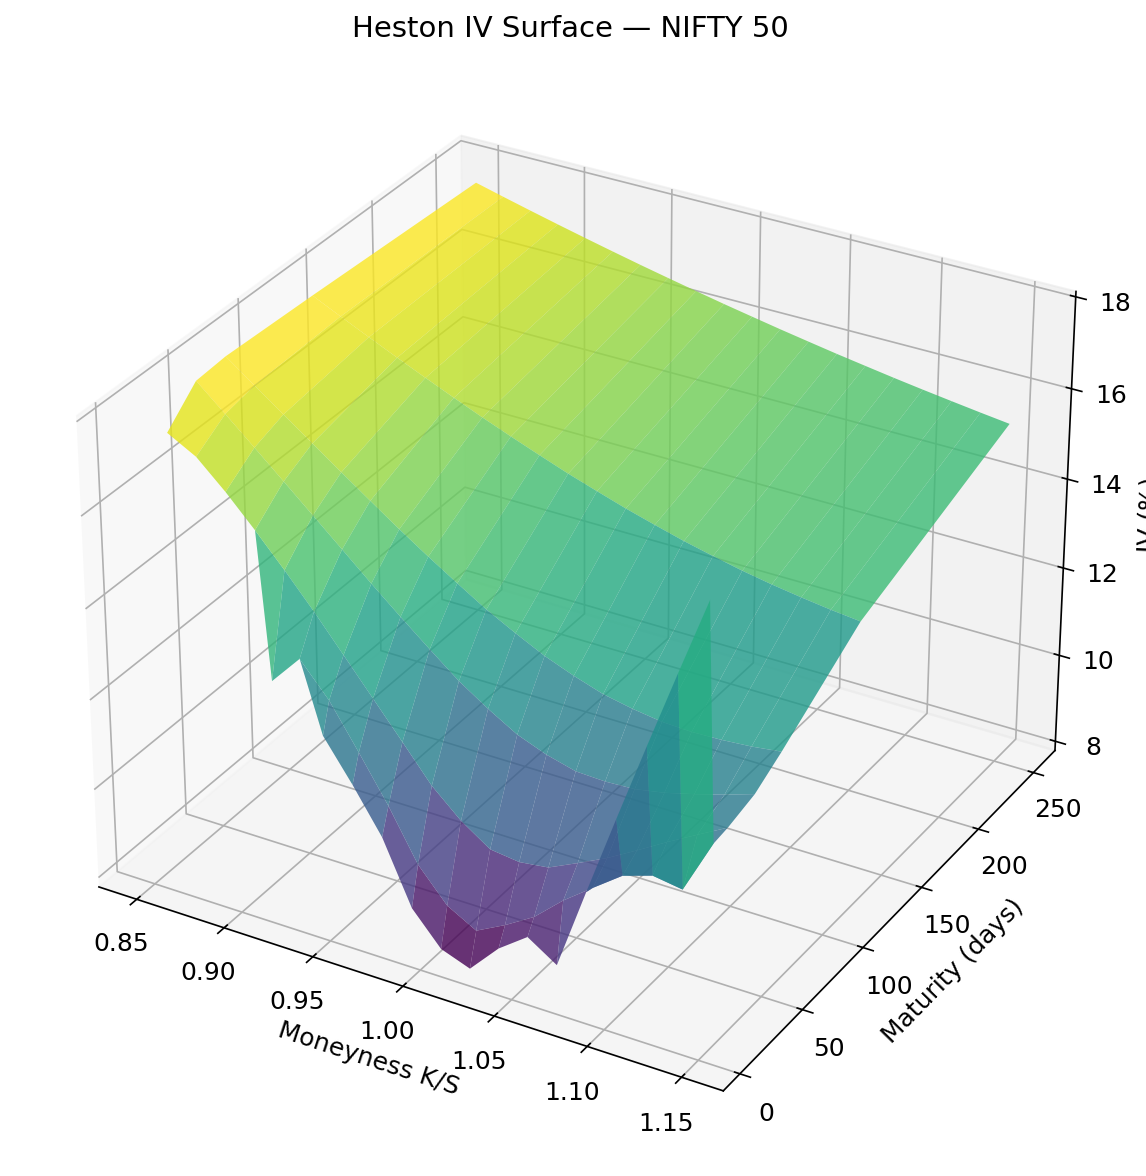
\includegraphics[width=\textwidth]{09_iv_surface_heston.png}\\[-2pt]
{\small\textbf{Heston IV Surface}}
\end{center}
\end{column}
\begin{column}{0.48\textwidth}
\begin{center}
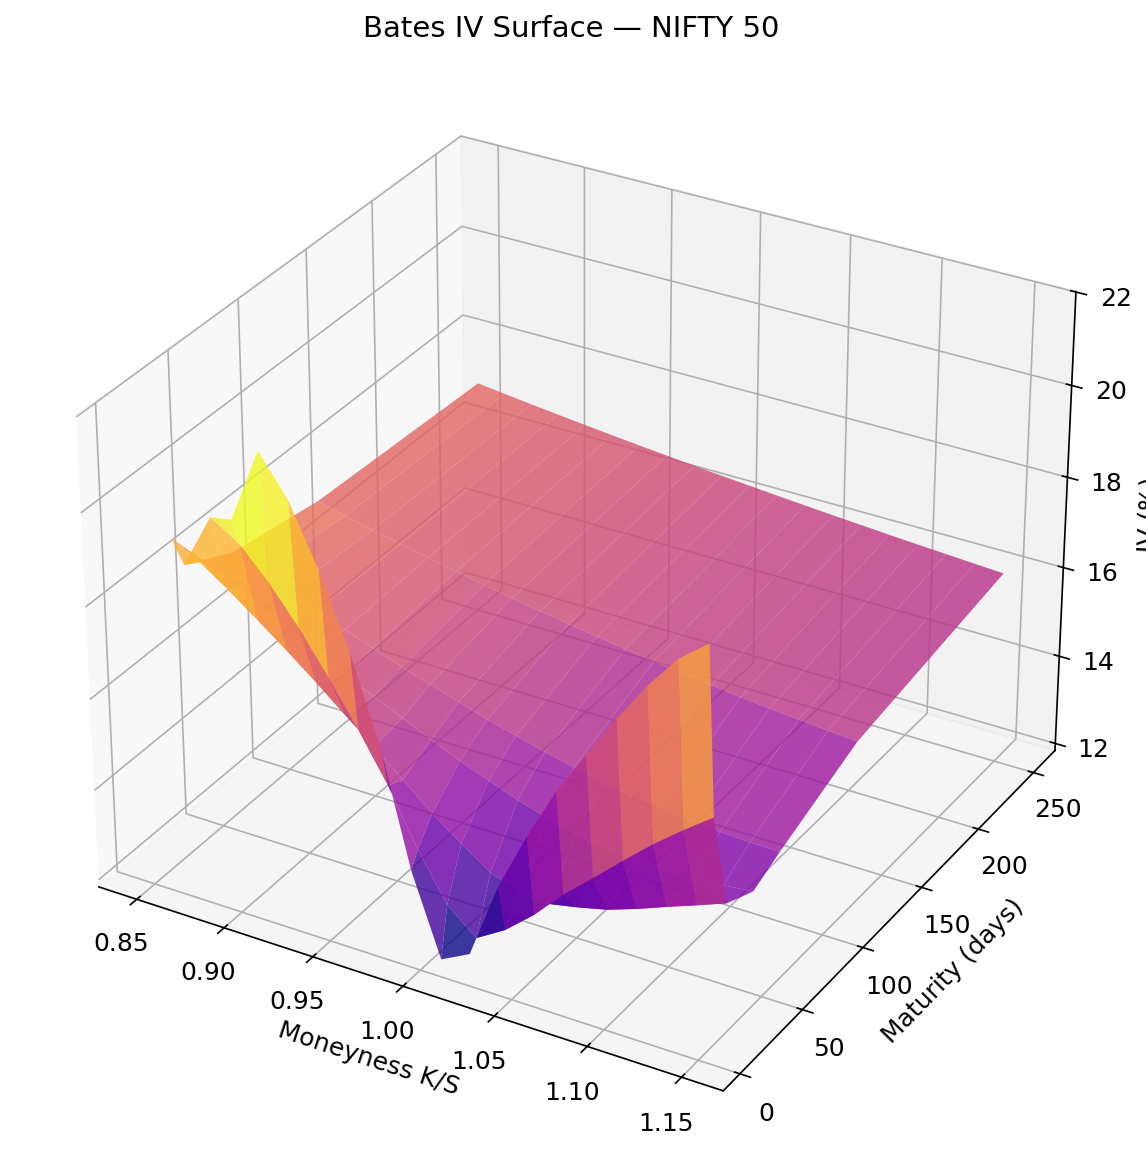
\includegraphics[width=\textwidth]{10_iv_surface_bates.png}\\[-2pt]
{\small\textbf{Bates IV Surface}}
\end{center}
\end{column}
\end{columns}
\vspace{3pt}
\small
Full IV surface (moneyness $\times$ maturity) generated from calibrated NIFTY parameters via Carr--Madan FFT. Bates produces richer short-maturity skew due to jumps. Both exhibit smile flattening at long maturities, converging to $\sqrt{\theta}$.
\end{frame}

% ===== SLIDE 17 =====
\begin{frame}{Heston \& Bates: Simulated Price and Volatility Paths}
\begin{columns}[c]
\begin{column}{0.48\textwidth}
\begin{center}
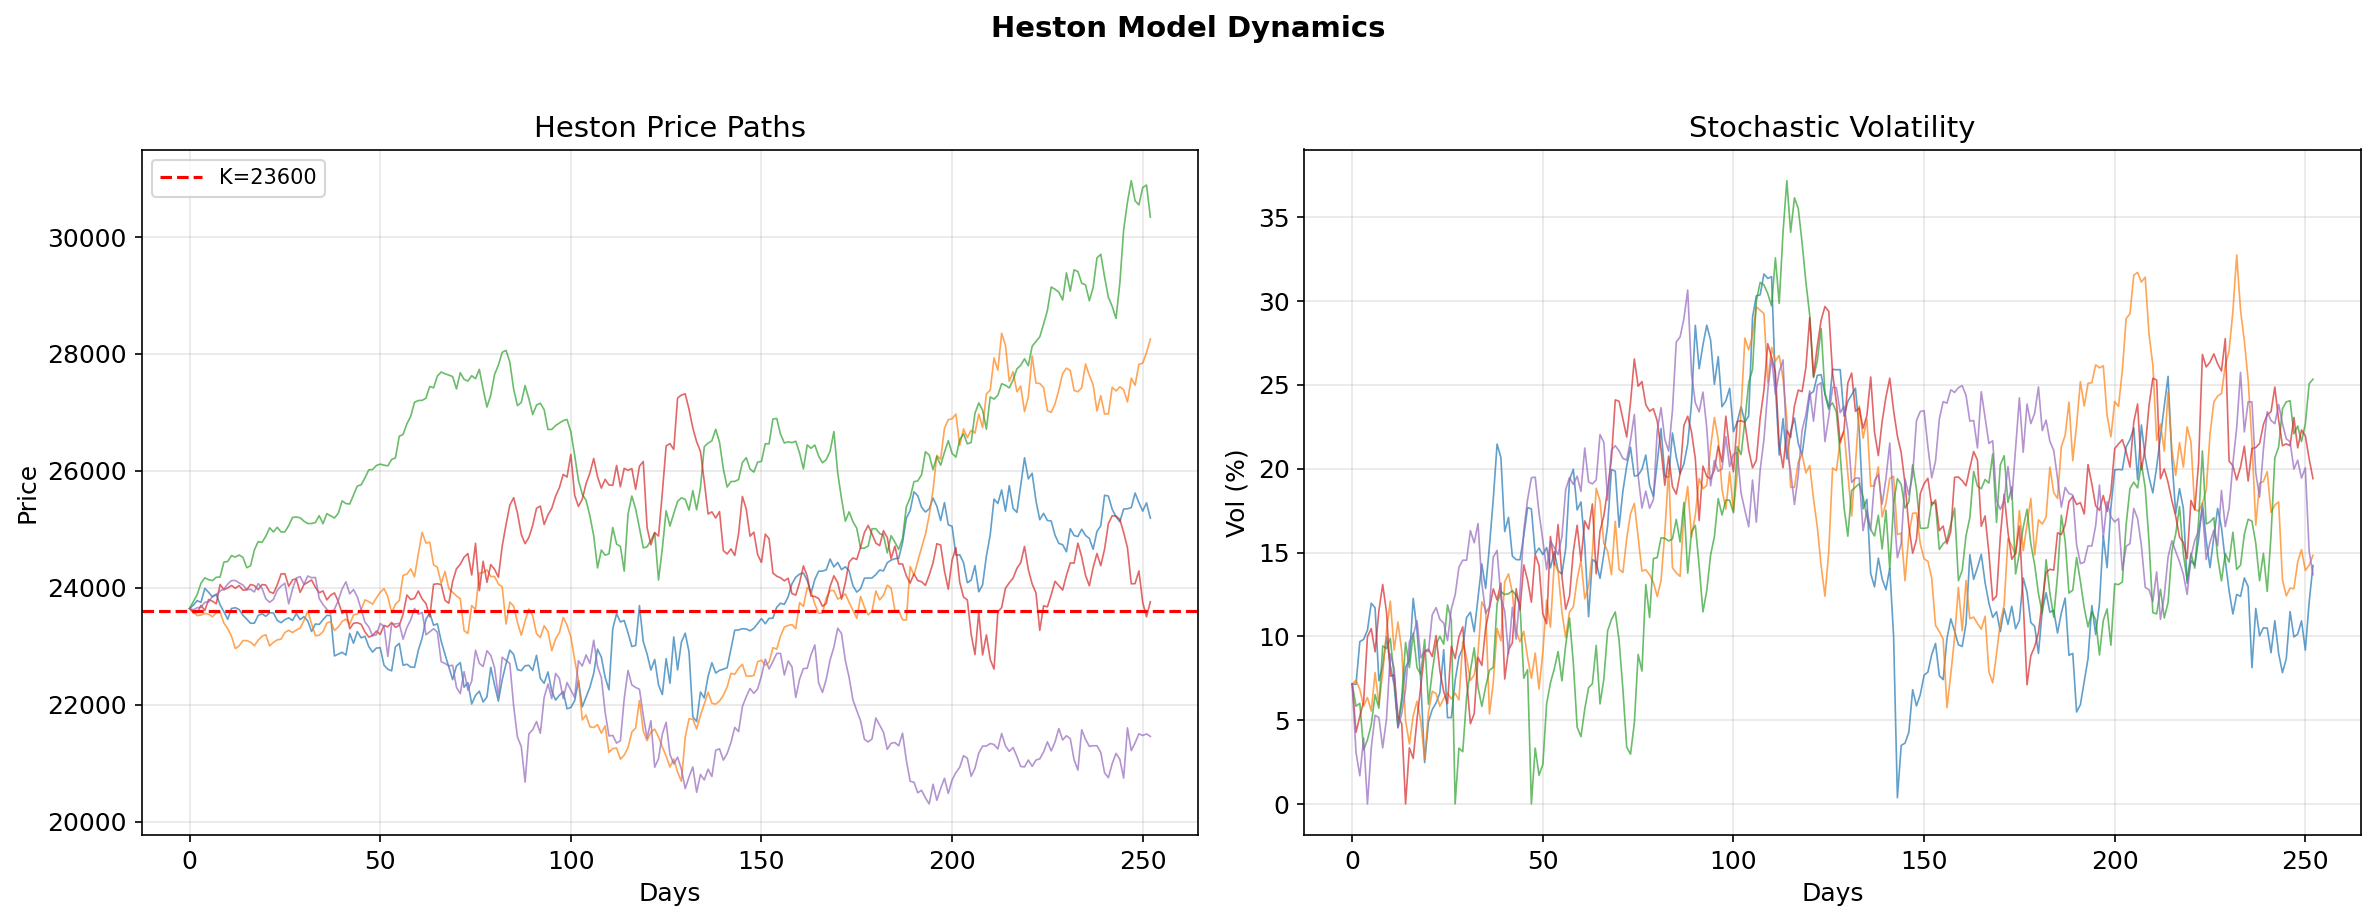
\includegraphics[width=\textwidth]{08_heston_paths.png}\\[-2pt]
{\small\textbf{Heston} --- smooth paths, stochastic vol}
\end{center}
\end{column}
\begin{column}{0.48\textwidth}
\begin{center}
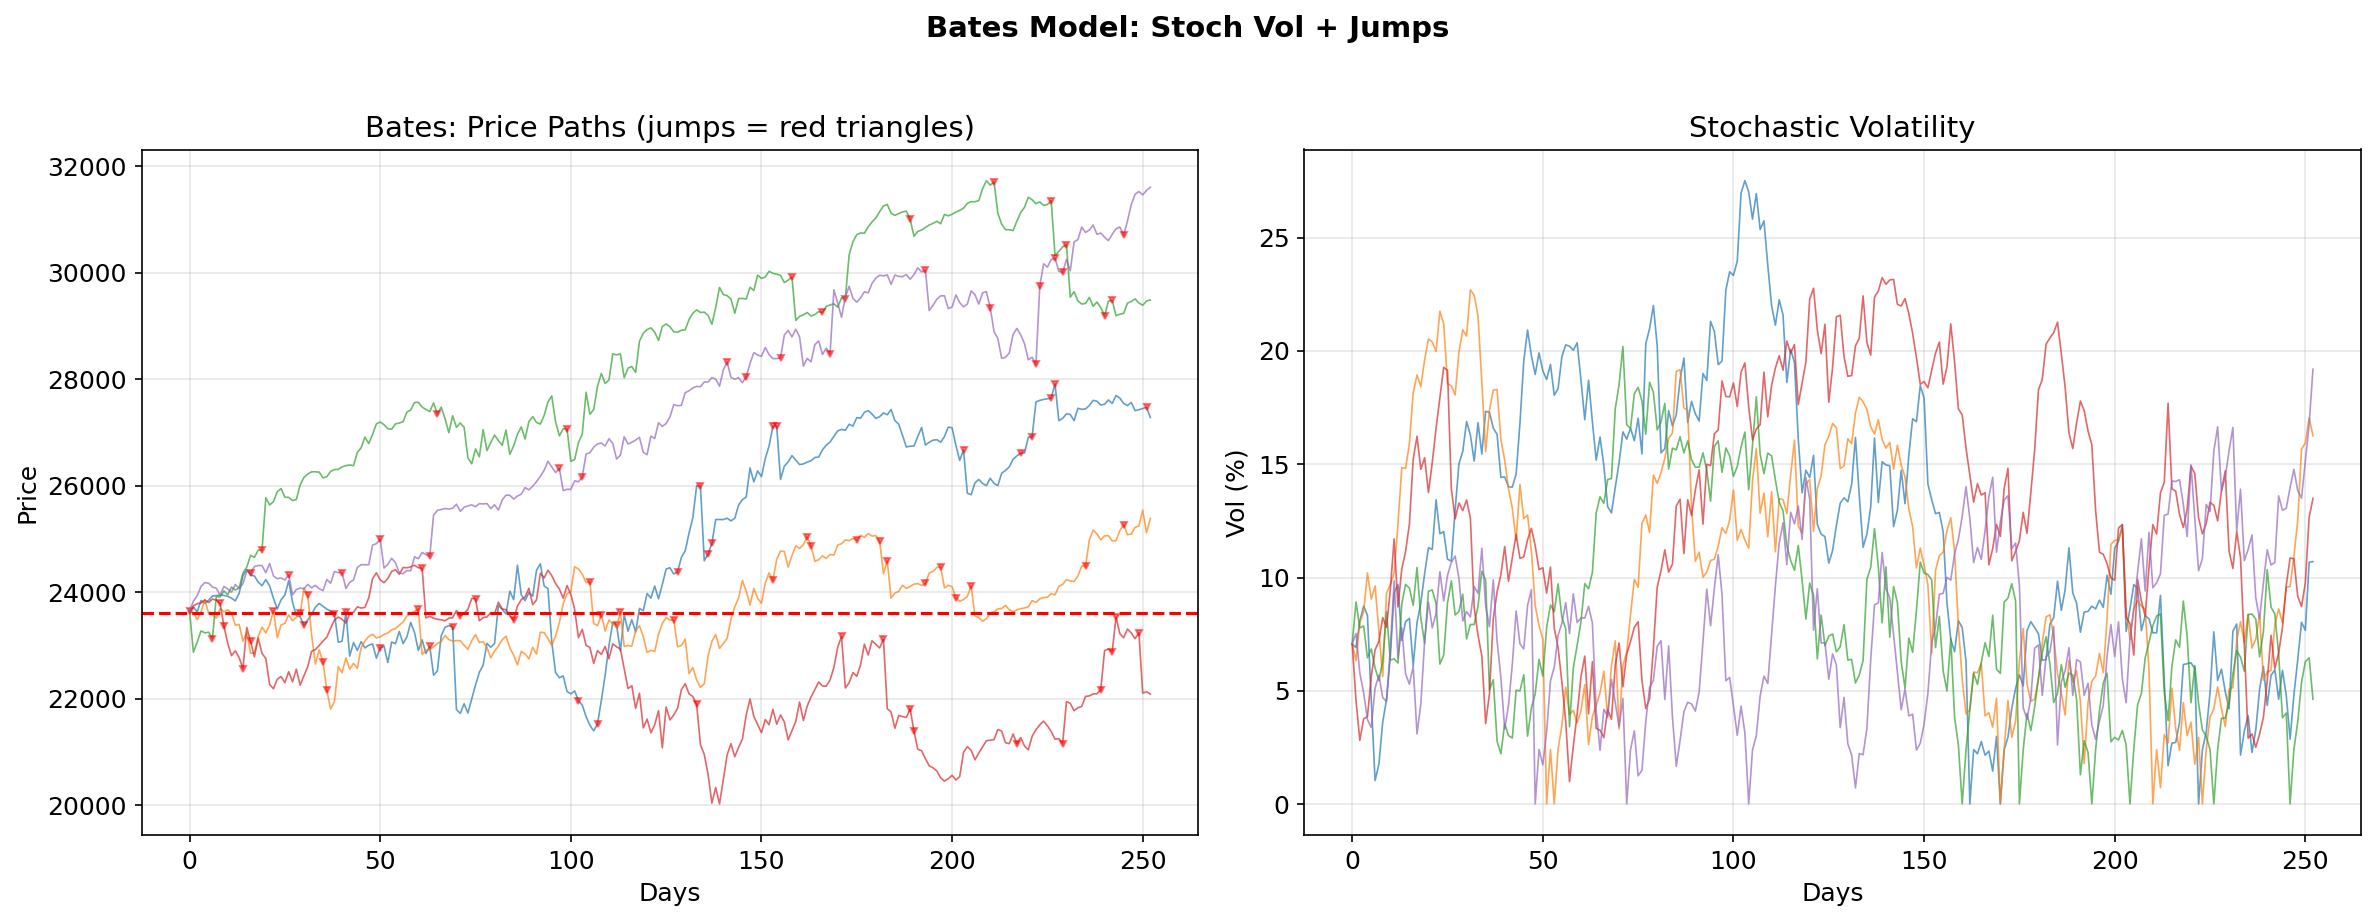
\includegraphics[width=\textwidth]{11_bates_paths.png}\\[-2pt]
{\small\textbf{Bates} --- jumps (red $\triangledown$) + stochastic vol}
\end{center}
\end{column}
\end{columns}
\vspace{3pt}
\small
Euler--Maruyama simulation with NIFTY-calibrated parameters (full truncation for $v_t \geq 0$). Bates paths show discrete price jumps overlaid on stochastic volatility clustering --- both features observed in real NIFTY data during crises (COVID, IL\&FS, elections).
\end{frame}

% ===== SLIDE 18 =====
\begin{frame}{OTM Put Pricing \& ATM Term Structure}
\begin{columns}[T]
\begin{column}{0.50\textwidth}
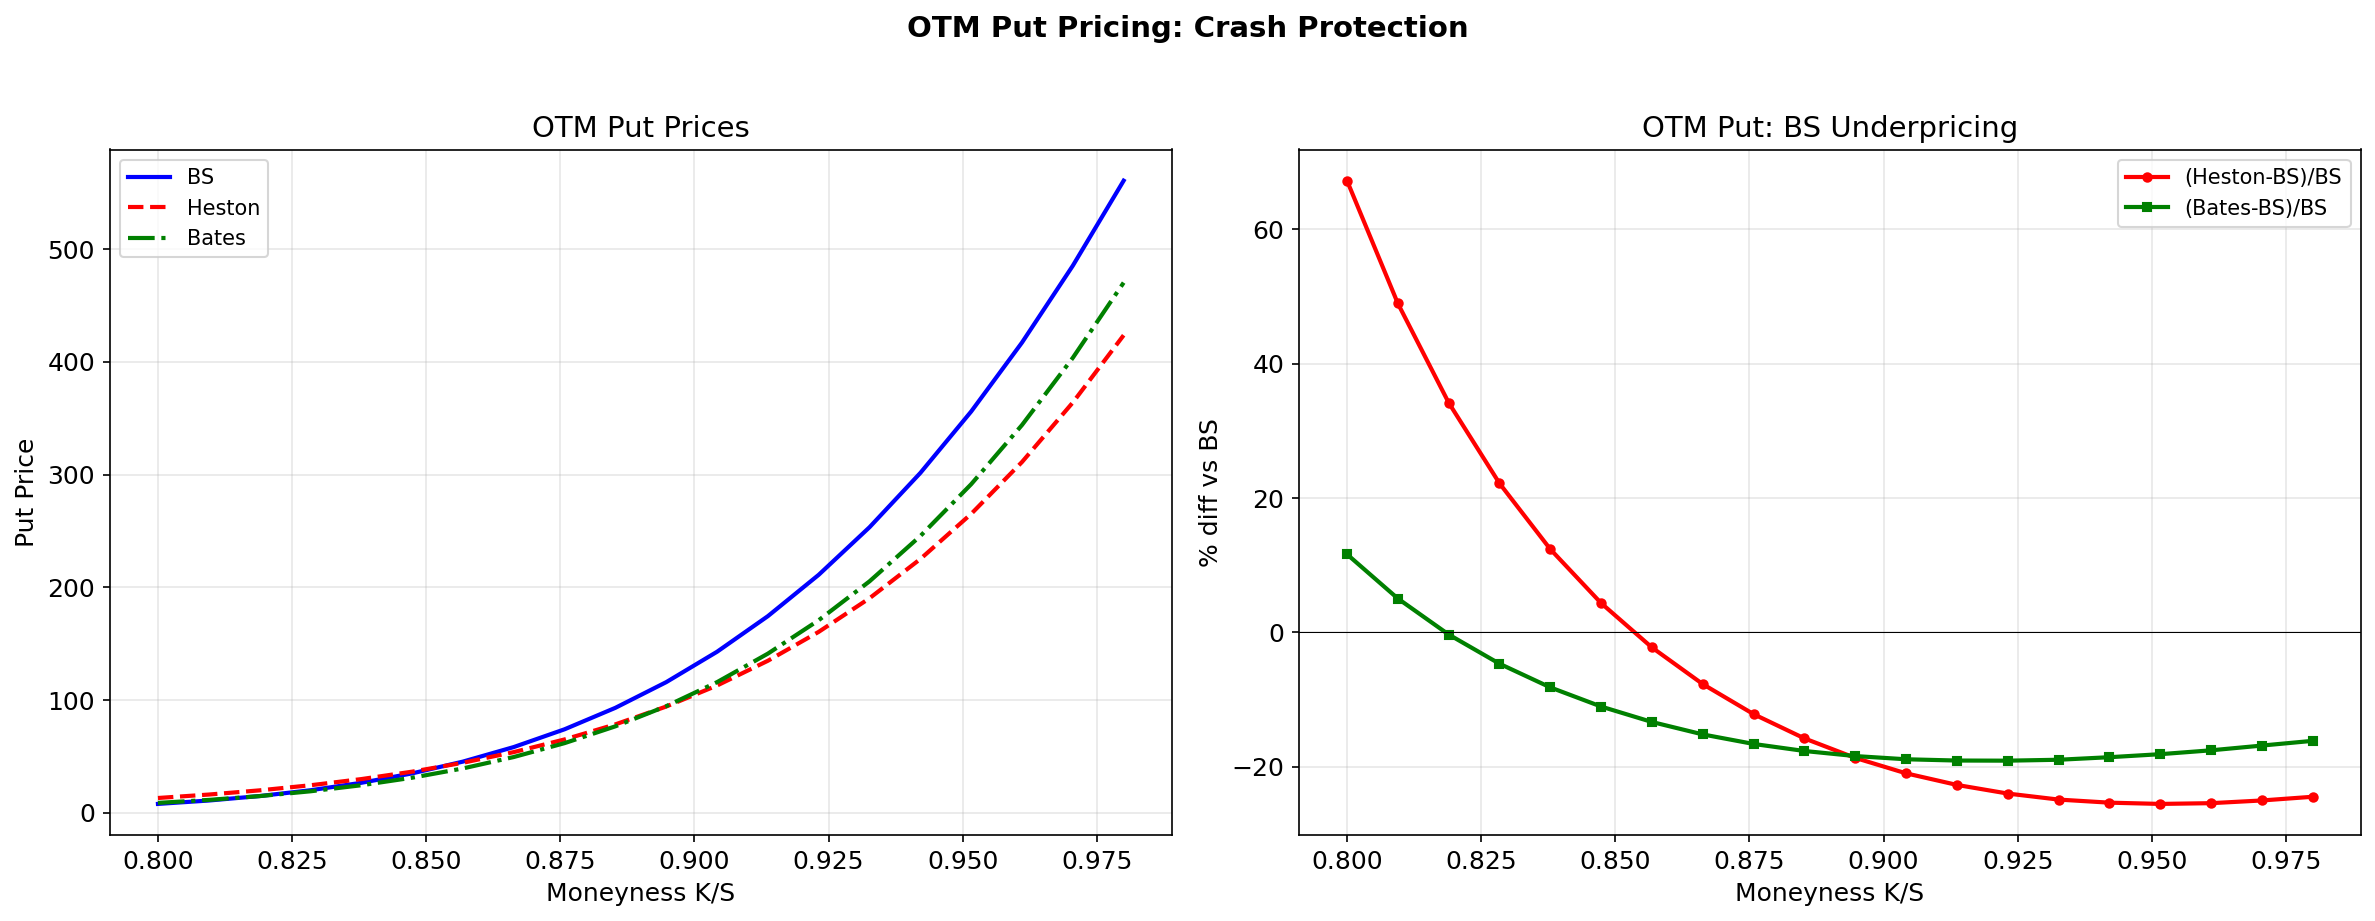
\includegraphics[width=\textwidth]{07_otm_puts.png}
\vspace{-3pt}
\footnotesize
\textbf{OTM puts} ($K/S_0 < 0.98$): Heston and Bates price crash protection \textbf{significantly higher} than BS. The \% difference grows as options become deeper OTM, exactly where crash risk matters most.
\end{column}
\begin{column}{0.48\textwidth}
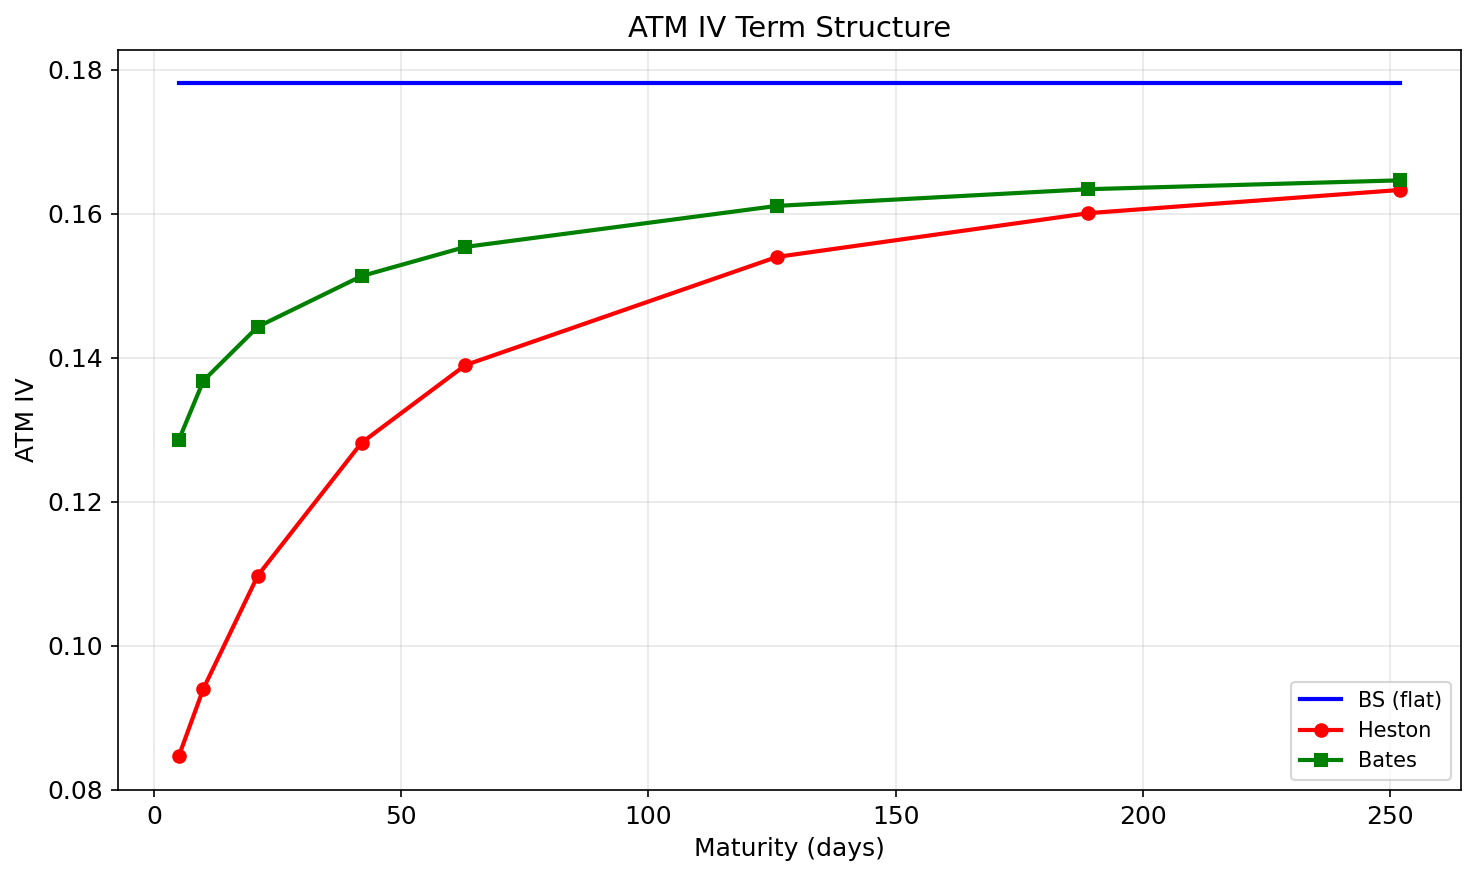
\includegraphics[width=\textwidth]{12_atm_term_structure.png}
\vspace{-3pt}
\footnotesize
\textbf{ATM IV term structure:} BS gives a flat line. Heston/Bates IV varies with maturity --- starts near $\sqrt{v_0} \approx 7\%$ and converges to $\sqrt{\theta} \approx 17\%$. This term structure is impossible under constant-vol models.
\end{column}
\end{columns}
\end{frame}

% ===== SECTION 6 =====
\section{Conclusions \& Future Work}

% ===== SLIDE 19 =====
\begin{frame}{Conclusions}
\begin{enumerate}\setlength\itemsep{3pt}
  \item \textbf{Four models calibrated on NIFTY 50:} BS $\subset$ MJD, Heston $\subset$ Bates.
    \begin{itemize}
      \item \textbf{Bates wins on AIC/BIC} (LL$=5610$, AIC$=-11205$) --- both stochastic vol and jumps are needed.
      \item $\rho = -0.39$ confirms leverage effect; $\mu_J < 0$ confirms crash-biased jumps.
    \end{itemize}
  \item \textbf{CFFT method} (Gao \& Hyndman 2025) implemented and validated:
    \begin{itemize}
      \item Stable CF (Thm~2.1) eliminates branch-cut discontinuities.
      \item Analytical error bounds (Thm~3.1): $|e| \leq \mathcal{O}(e^{-cN}) + \mathcal{O}(N^{-2})$ --- verified on NIFTY data.
      \item CFFT-II achieves comparable accuracy to Carr--Madan at $\sim$half the grid size.
    \end{itemize}
  \item \textbf{Option pricing results:}
    \begin{itemize}
      \item BS underprices OTM puts by 20--100\%+ (consistent across all advanced models).
      \item Heston/Bates produce full IV surface --- smile + term structure.
      \item Bates captures both stochastic vol clustering and discrete crash events observed in NIFTY.
    \end{itemize}
\end{enumerate}

\vspace{3pt}
\textbf{Future:} Calibrate to live NSE option chain; tamed Milstein MC [KS19]; regime-switching [KK20]; exotic options via CFFT backward induction.
\end{frame}

% ===== SLIDE 20 =====
\begin{frame}[allowframebreaks]{References}
\footnotesize
\begin{enumerate}\setlength\itemsep{1pt}
  \item Black, F.\ \& Scholes, M.\ (1973). The Pricing of Options and Corporate Liabilities. \emph{JPE} 81(3).
  \item Merton, R.\ (1976). Option pricing when underlying stock returns are discontinuous. \emph{JFE} 3(1--2).
  \item Heston, S.L.\ (1993). A closed-form solution for options with stochastic volatility. \emph{RFS} 6(2).
  \item Bates, D.\ (1996). Jumps and stochastic volatility. \emph{RFS} 9(1).
  \item Carr, P.\ \& Madan, D.\ (1999). Option valuation using the fast Fourier transform. \emph{J.\ Comp.\ Finance} 2(4).
  \item Kahl, C.\ \& J\"ackel, P.\ (2005). Not-so-complex logarithms in the Heston model. \emph{Wilmott} 19(9).
  \item Lord, R.\ et al.\ (2008). A fast FFT-based method for pricing under L\'evy processes. \emph{SIAM J.\ Sci.\ Comp.} 30(4).
  \item \textbf{Gao, X.\ \& Hyndman, C.\ (2025).} Convolution-FFT for option pricing in the Heston model. \emph{arXiv:2512.05326}.
  \item Dareiotis, Kumar \& Sabanis (2016). Tamed Euler for L\'evy SDEs. \emph{SIAM J.\ Numer.\ Anal.} 54(3).
  \item Kumar \& Sabanis (2019). Milstein with super-linear diffusion. \emph{BIT} 59(4).
  \item Kumar \& Kumar (2020). Tamed Milstein for Markovian switching. \emph{JCAM} 377.
  \item A\"it-Sahalia (2002). MLE of discretely sampled diffusions. \emph{Econometrica} 70(1).
  \item Iacus (2008). \emph{Simulation and Inference for SDEs}. Springer.
  \item Glasserman (2003). \emph{Monte Carlo Methods in Financial Engineering}. Springer.
\end{enumerate}
\end{frame}

% ===== SLIDE 21 =====
\begin{frame}
\centering
\vfill
{\Huge\bfseries Thank You}\\[12pt]
{\Large Questions?}
\vfill
\end{frame}

\end{document}
